
\documentclass[dvipdfmx]{standalone}
\usepackage[T1]{fontenc}
\usepackage{newtxtext, newtxmath}

\usepackage{tikz}
\usetikzlibrary{positioning}

\begin{document}
  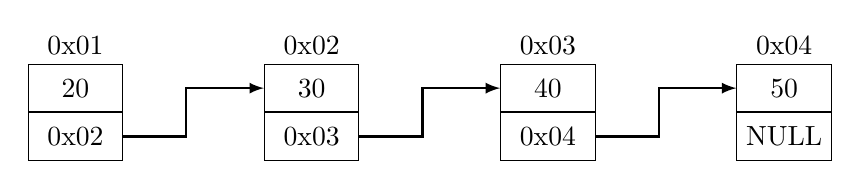
\begin{tikzpicture}[> = latex]
    \tikzset{
      block/.style={
        draw, rectangle, minimum width=1.2cm, minimum height=0.6cm,
      }
    }
    % blocks
    \foreach[count=\i] \addr\data\nextaddr in {0x01/20/0x02, 0x02/30/0x03, 0x03/40/0x04, 0x04/50/NULL} {
      \draw (\i*3,0) node (elem\i data) [block] {\data} node[above=3mm] {\addr};
      \node (elem\i next) [block, below=0mm of elem\i data] {\nextaddr};
    }
    % % arrows
    \foreach \from\to in {1/2, 2/3, 3/4} {
      \draw[->, thick] (elem\from next.east) -- ++(right:0.8cm) |- (elem\to data);
    }

  \end{tikzpicture}
\end{document}
